\begin{activity} \label{A:7.2.1}  
  Consider the autonomous differential equation 
$$
\frac{dy}{dt} = -\frac 12( y - 4).
$$

\ba
\item Make a plot of $\frac{dy}{dt}$ versus $y$ on the axes provided.  Looking at the
  graph, for what values of $y$ does $y$ increase and for what values of $y$
  does $y$ decrease?

  \begin{center}
    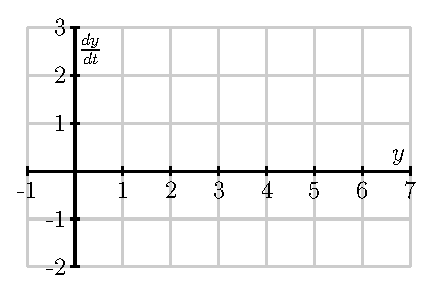
\includegraphics{figures/7_2_Act1_1.eps}
  \end{center}

\item Next, sketch the slope field for this differential equation on the axes provided.

  \begin{center}
    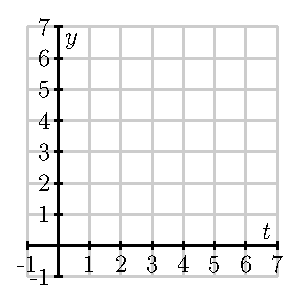
\includegraphics{figures/7_2_Act1_2.eps}
  \end{center}

\item  Use your work in (b) to sketch the solutions that satisfy $y(0) = 0$, $y(0) = 2$, $y(0) = 4$ 
  and $y(0) = 6.$

\item  Verify that $y(t) = 4 + 2e^{-t/2}$ is a solution to the given
  differential equation with the initial value $y(0) = 6.$  Compare
  its graph to the one you sketched in (c).

\item  What is special about the solution where $y(0) = 4$?  

\ea
\end{activity}
\begin{smallhint}
\ba
	\item Small hints for each of the prompts above.
\ea
\end{smallhint}
\begin{bighint}
\ba
	\item Big hints for each of the prompts above.
\ea
\end{bighint}
\begin{activitySolution}
\ba
	\item Solutions for each of the prompts above.
\ea
\end{activitySolution}
\aftera